% The preceding line is only needed to identify funding in the first footnote. If that is unneeded, please comment it out.
\documentclass[conference]{IEEEtran}
\usepackage{fontspec}
\usepackage{tikz}
\usepackage{amsmath,amssymb,amsfonts}
\usepackage{algorithmic}
\usepackage{graphicx}
\usepackage{textcomp}
\usepackage{xcolor} 
\usepackage{comment}
\usepackage{booktabs}


\def\BibTeX{{\rm B\kern-.05em{\sc i\kern-.025em b}\kern-.08em
    T\kern-.1667em\lower.7ex\hbox{E}\kern-.125emX}}
\usepackage[numbers,sort&compress]{natbib}


% Some colors
\definecolor{c1}{RGB}{84, 156, 22}
\definecolor{c2}{RGB}{190, 214, 71}
\definecolor{c3}{RGB}{237, 163, 52}
\definecolor{c4}{RGB}{194, 36, 21}

\begin{document}

\title{How Does the Level of Somatosensory Feedback Fidelity Impact Motor Learning in VR: \\a Systematic Review}

\author{\IEEEauthorblockN{Reinprecht Christian}
\IEEEauthorblockA{TU Delft, NL \\
C.T.Reinprecht@student.tudelft.nl}
\and
\IEEEauthorblockN{Ratschat Alex}
\IEEEauthorblockA{TU Delft, NL \\
A.L.Ratschat@tudelft.nl}
\and
\IEEEauthorblockN{Marchal-Crespo Laura}
\IEEEauthorblockA{TU Delft, NL \\
L.MarchalCrespo@tudelft.nl}
}

\maketitle

\begin{abstract}
The abstract will come here.
\end{abstract}

\begin{IEEEkeywords}
motor learning, fidelity, virtual reality, systematic review
\end{IEEEkeywords}

%%%%% INTRODUCTION %%%%%
\section{Introduction}

Simulations in virtual reality (VR) provide a comprehensive platform for users to acquire new skills and competencies, with applications ranging from physical therapy and rehabilitation to sports and industrial training, education, marketing, telerobotics, and research, as well as gaming and entertainment \cite{Wu2023TrainingReality, Oagaz2022PerformanceReality}. Furthermore, the virtual environment (VE) allows for the studying of complex skills, as well as the evaluation of the user's performance without giving up on experimental control, which facilitates the understanding of motor learning on a level that is not possible in the physical world \cite{Harris2021ExploringSimulator, Levac2019LearningReview}. Therefore it is not surprising that there is a great interest in VR-based training simulations, especially to teach skills that would otherwise have to be acquired in dangerous or sensitive environments, such as construction work, military training, or surgical operations \cite{Adami2021EffectivenessTeleoperation, Lele2013VirtualUtility, Qi2021VirtualScenario}.

When interacting with real-world objects, we rely not only on visual feedback but also on information obtained through the mechanoreceptors in our skin and muscles \cite{Gonzalez-Grandon2021ProprioceptionInteraction}. To provide these stimuli in the virtual world, tools or devices are required to reproduce the sensations we would expect when interacting with objects in the VE, which includes the perception of pressure, vibration, temperature, and the position and movement of body parts. Exposing the user to these sensations when they are interacting with objects in VR --- generally denoted as somatosensory feedback --- may offer a promising approach to increase the effectiveness of motor learning \cite{Sainburg2022MovementNeurorehabilitation, Sigrist2013AugmentedReview}.
The degree to which the feedback in the VE mimics real-world interaction is determined by its fidelity \cite{Caird1996PersistentTraining}, which ranges from simple, binary cues such as vibration to high-fidelity feedback that feels as if the user is interacting with a real object \cite{Yang2023TheSimulation}.

% Teasing the research topic
While researchers previously assumed that higher fidelity correlates with better training performance in VR \cite{Caird1996PersistentTraining, Waller1998TheTraining}, as the interaction feels more natural, recent research suggests that there might be no linear correlation between the level of fidelity and motor performance: Instead, motor performance decreased in conditions that yielded mid-fidelity, compared to scenarios with high fidelity and well-designed low fidelity \cite{MahdiNabiyouni201520153DUI.}.

However, regarding task complexity, using a mid-fidelity controller may be beneficial, as it has been shown to effectively reduce the task load in a drilling task \cite{Yang2023TheSimulation}. This might be valuable for the motor learning performance of people with impaired motor skills \cite{Sigrist2013AugmentedReview}, aligning with the challenge point framework which states that less skilled subjects might not advance if the performed task is too demanding \cite{Guadagnoll2004ChallengeLearning}. 

% Added reviews, second round of going to research gap
Extensive reviews have been conducted to illuminate the impact of haptic feedback in VR-based training \cite{Sigrist2013AugmentedReview} and the general utility of haptic simulation in motor learning \cite{Al-Saud2021TheReview}. However, it remains unclear how exactly different levels of haptic feedback fidelity affect motor learning, and to our knowledge, it has not been disentangled which kinds of tasks to be learned necessitate which degree of feedback accuracy.
Since supplying high fidelity to a VE is very costly, it is important to determine under which circumstances low-fidelity feedback, such as through somatosensory cues, is sufficient to increase the effectiveness of motor learning, and where high-fidelity feedback is necessary. 

In this work, we systematically review current research to create an overview of the impact of different levels of somatosensory feedback fidelity on motor learning in VR. Furthermore, this review will address how the level of feedback fidelity may affect the transfer of the learned skills to the real environment.

We hypothesize that in complex movements that necessitate precise timing for the correct execution of the task, such as ballistic movements, a high level of somatosensory feedback fidelity may be beneficial for motor learning. However, low-fidelity feedback may be sufficient for enhancing motor learning performance in scenarios involving constant movement velocities, allowing for reduced system cost and simpler experimental design. \newpage


%%%%% METHODS %%%%%
\section{Methods}

\subsection{Search strategy and data sources}
Several relevant articles were reviewed at the beginning to find eligible search terms. The query based on the research question consists of three main parts, namely \textit{virtual reality}, \textit{somatosensory feedback}, and \textit{motor learning}, each term with their respective synonyms. 

The final search query was as follows: motor AND (learning OR control OR training OR skills) AND (((virtual OR augmented) AND reality) OR ((remote OR virtual OR simulated) AND environment)) AND (((somatosensory OR haptic OR tactile OR proprioceptive OR kinesthetic OR cutaneous OR somatic) AND 
(cue* OR feedback OR rendering OR stimul*)) AND (fidelity OR realism OR accuracy OR precision OR exactness OR specificity)). The search terms were applied for the article title, abstract, and keywords.

Three databases (Scopus, IEEE Xplore, and PubMed) were searched in April 2024. Based on the required syntax of each database, the search query was slightly adapted. For example, as PubMed only allows for the use of an asterisk for words containing more than three letters, the term \textit{cue*} was changed to (\textit{cue} OR \textit{cues}). The exact search queries can be found in \ref{sec:queries}. 

\subsection{Study Selection}
The search results were saved in Mendeley. Duplicate publications were identified and removed. Following the PRISMA method \cite{Page2021TheReviews}, the found results were first screened based on their title and abstract and then reviewed in full length (see fig. \ref{fig:prisma}). Records were excluded based on the exclusion criteria in \ref{sec:exclusion}.

\section{Results}

The search yielded a total of 329 results.

\begin{figure}[ht]
    \centering
    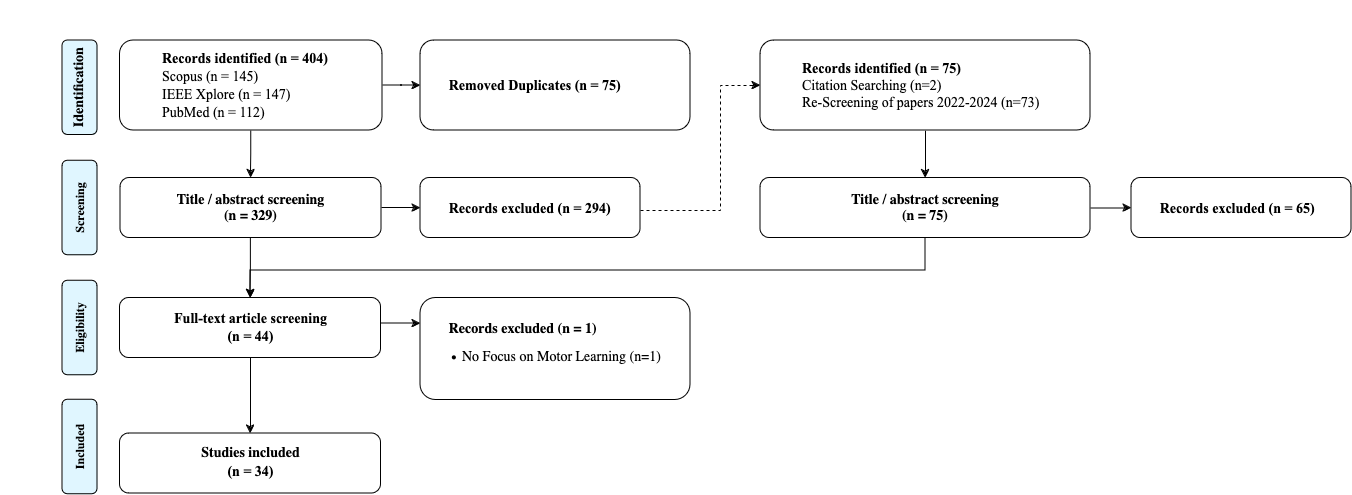
\includegraphics[width=\columnwidth]{prisma_overview.png} 
    \caption{Overview of the methodology using the PRISMA method}
    \label{fig:prisma}
\end{figure}



\subsection{Eligibility criteria}
\label{sec:eligibility}
\subsubsection{Inclusion criteria}
To be eligible for inclusion, studies needed to focus on the impact of haptic and/or somatosensory feedback on motor learning in humans. There were no publication date or language limits. We included studies with healthy participants only, as patients often know how to perform a movement but are physically constrained by their condition, therefore augmented feedback may help the motor learning of patients in a different way compared to healthy subjects \cite{Sigrist2013AugmentedReview}.

\subsubsection{Exclusion criteria}
\label{sec:exclusion}
Records were considered not eligible for inclusion if they were or focused on:
\begin{itemize}
    \item Studies not related to motor learning in humans,
    \item Systems not providing haptic feedback in VR,
    \item Studies that focused on a neurological condition and its implications for motor learning,
    \item Studies explaining a new assessment system for the evaluation of motor learning,
    \item Studies of haptic guidance only.
\end{itemize}

\subsection{Other studies included}
A second screening of more recent papers (no older than 3 years) was done. 72 papers were re-screened, and 9 more papers were included.

\subsection{Study characteristics}

\subsubsection{Year of publication}
The year of publication of the included studies ranges from 2000 to 2024. As seen in \ref{fig:years}, the number of studies has greatly increased in the past decade, with a peak in 2018.

\begin{figure}[ht]
    \centering
    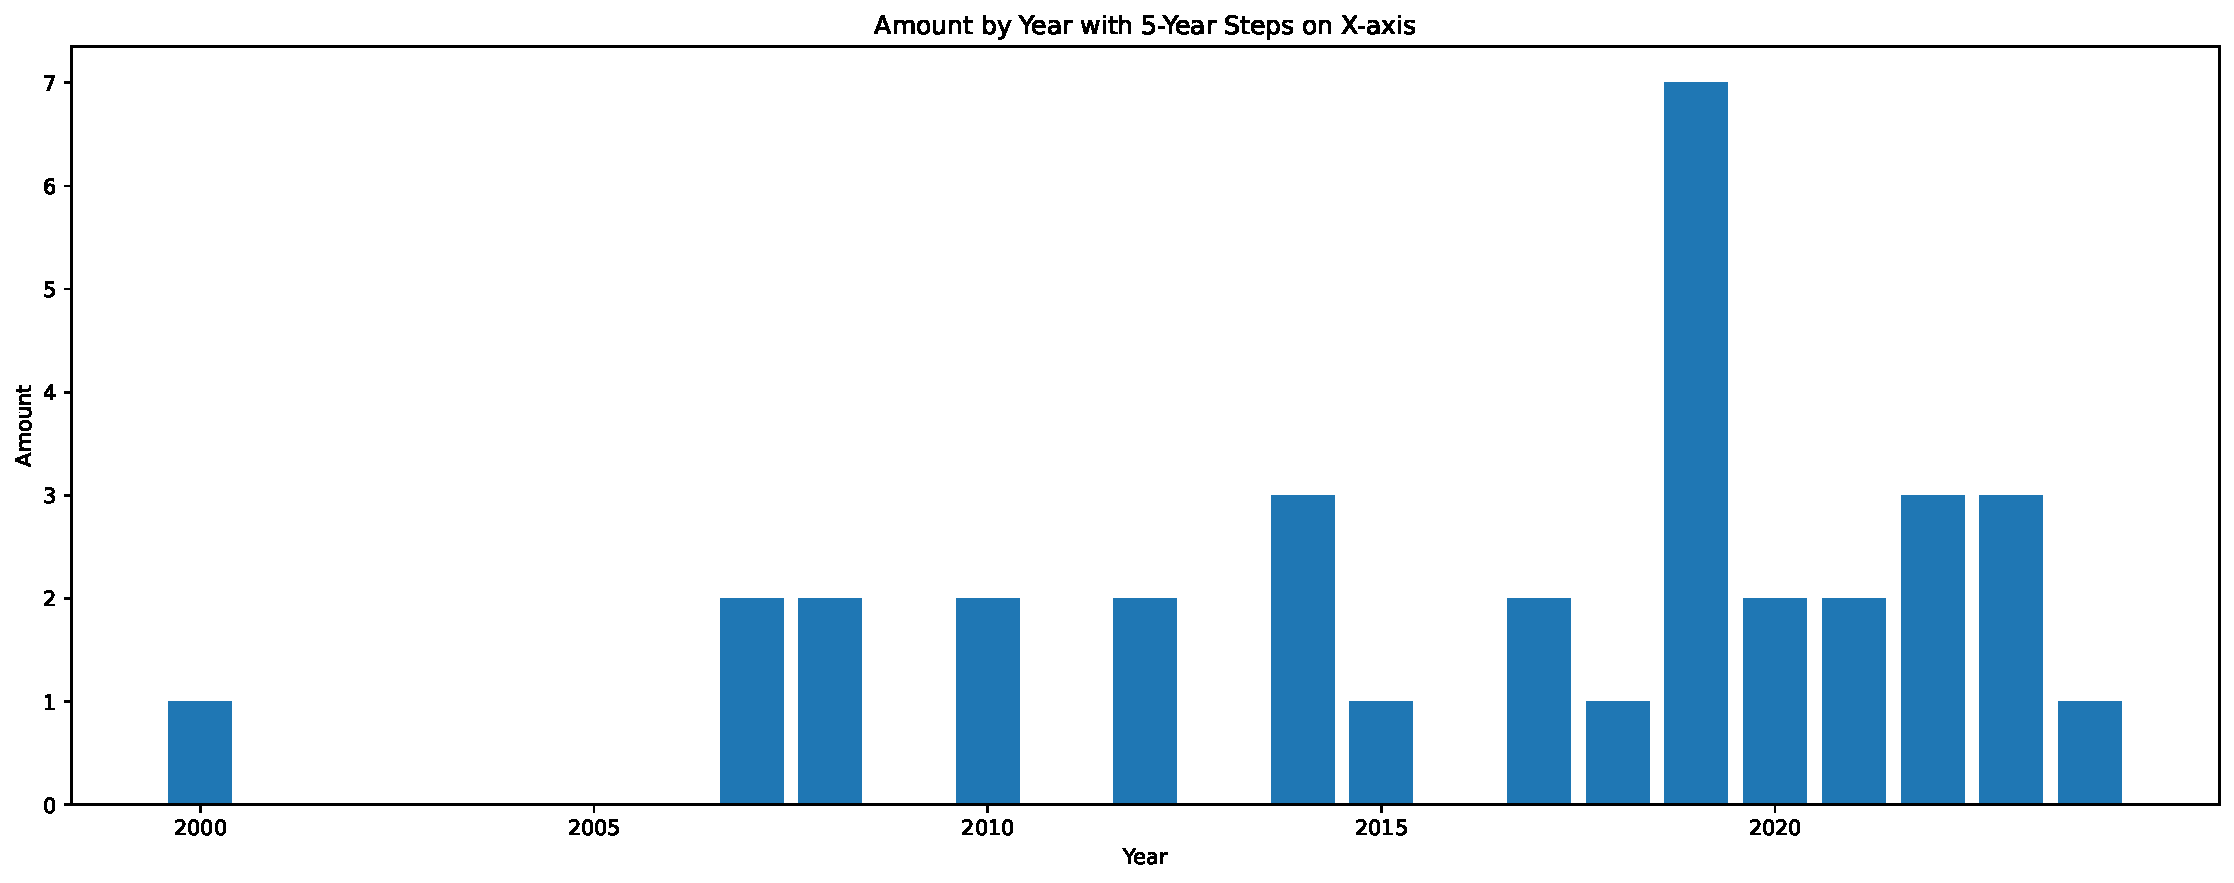
\includegraphics[width=\columnwidth]{years.pdf} 
    \caption{Publication dates of the included articles}
    \label{fig:years}
\end{figure}

\section{Definitions}
\subsection{Fidelity}
Huang et al. suggested that skill transfer might be a useful paradigm to evaluate the level of fidelity, assuming that if an environment has infinite fidelity and is therefore perfectly recreating the sensations of the real environment, then there would be no performance loss when transferring the skill from the virtual to the real environment \cite{Huang2006}

\section{Somatosensory feedback}
\subsection{Low-fidelity feedback}

\subsection{Mid-fidelity feedback}
Even though it is not labeled as such, Morris et al. conducted an experimental study in which they provided mid-fidelity feedback to the participants. They were asked to follow a trajectory with a haptic device stylus, and in the first condition of the experiment the device provided force feedback that was pointing in the opposite direction as the trajectory, while the participants were asked to keep the device in the movement plane, so to counteract the applied force exactly \cite{Morris2007}. While participants applied the same force necessary to follow the trajectory, the movement and position control differed from actually following the pattern.



\subsection{High-fidelity feedback}
Huang et al. showed in an experiment that high-fidelity feedback can be helpful in controlling an external dynamic system, as it enhances performance during online control \cite{Huang2007}. The subjects were asked to excite a spring-inertia system with maximum amplitude, which could be achieved by leveraging the resonance frequency of the system and therefore increasing its oscillations. When haptic feedback was provided, the participants were more precise in finding the frequency and decreased their variability.

Haptic guidance specifically can help in the temporal aspects of learning a task \cite{Feygin2002HapticSkill} 

\subsection{Framework}

\subsection{Hardware precision}
"The required refresh rate to provide realistic
force feedback is commonly accepted to be at least 1,000 Hz.
However, this refresh rate is widely debated. According to
Burdea [14], a minimum refresh rate of only 300 Hz is
acceptable. Conversely, a study by Booth et al. [15] using
SensAble’s Premium 1.5 to deduce the minimum acceptable
haptic refresh rate, suggests that “a minimum acceptable
refresh rate must lie within the 550-600 Hz range.” The
necessary rate of update is dependent upon the stiffness of
the surfaces to be simulated. A stiff contact between objects is
better simulated by higher refresh rates, whereas lower
refresh rates are satisfactory for softer objects. Additional
methods can be applied to simulate touching stiffer objects
such as combining vibrations with force to the end effector to
represent the small vibrations felt upon object contact [16].
Typically, a trade-off must be made between the accuracy of
the haptics effects produced and the speed required within
the application." \cite{Coles2011TheArt}
About latency and its impacts: \cite{Gourishetti2018PassiveFeedback}.
Ballistic movements: rapid, involuntary movement which is motor programmed, and for which visual feedback is not possible \cite{Wall2000}.

\section{Results}

\begin{figure}[ht]
    \centering
    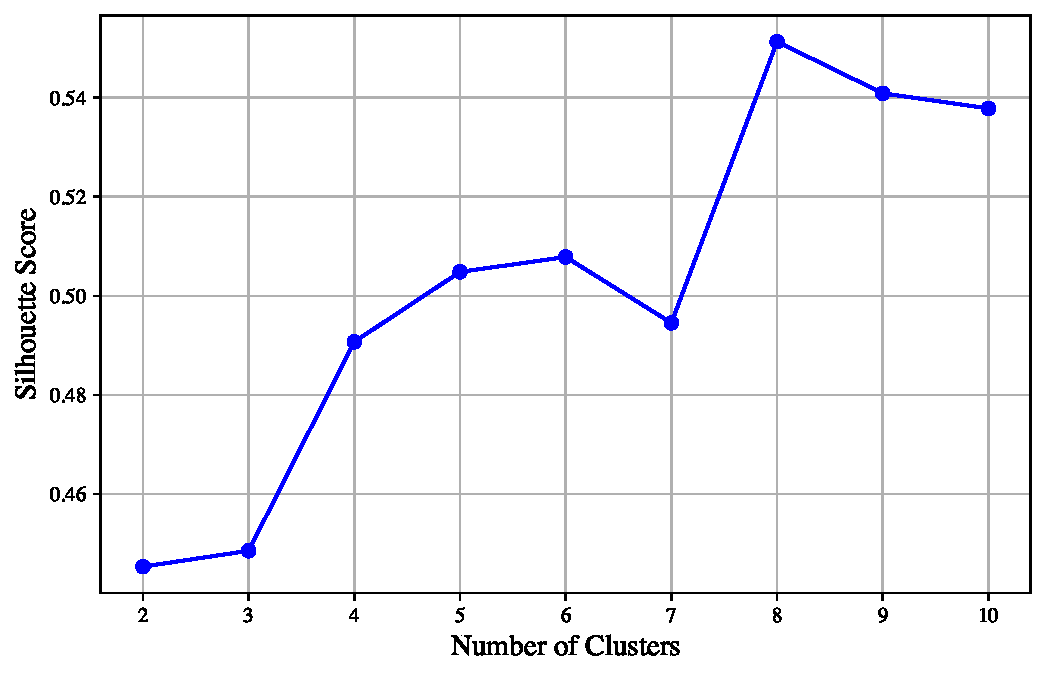
\includegraphics[width=\columnwidth]{silhouette.pdf} 
    \caption{Silhouette scores for the numbers of clusters}
    \label{fig:silhouette}
\end{figure}

\begin{figure}[ht]
    \centering
    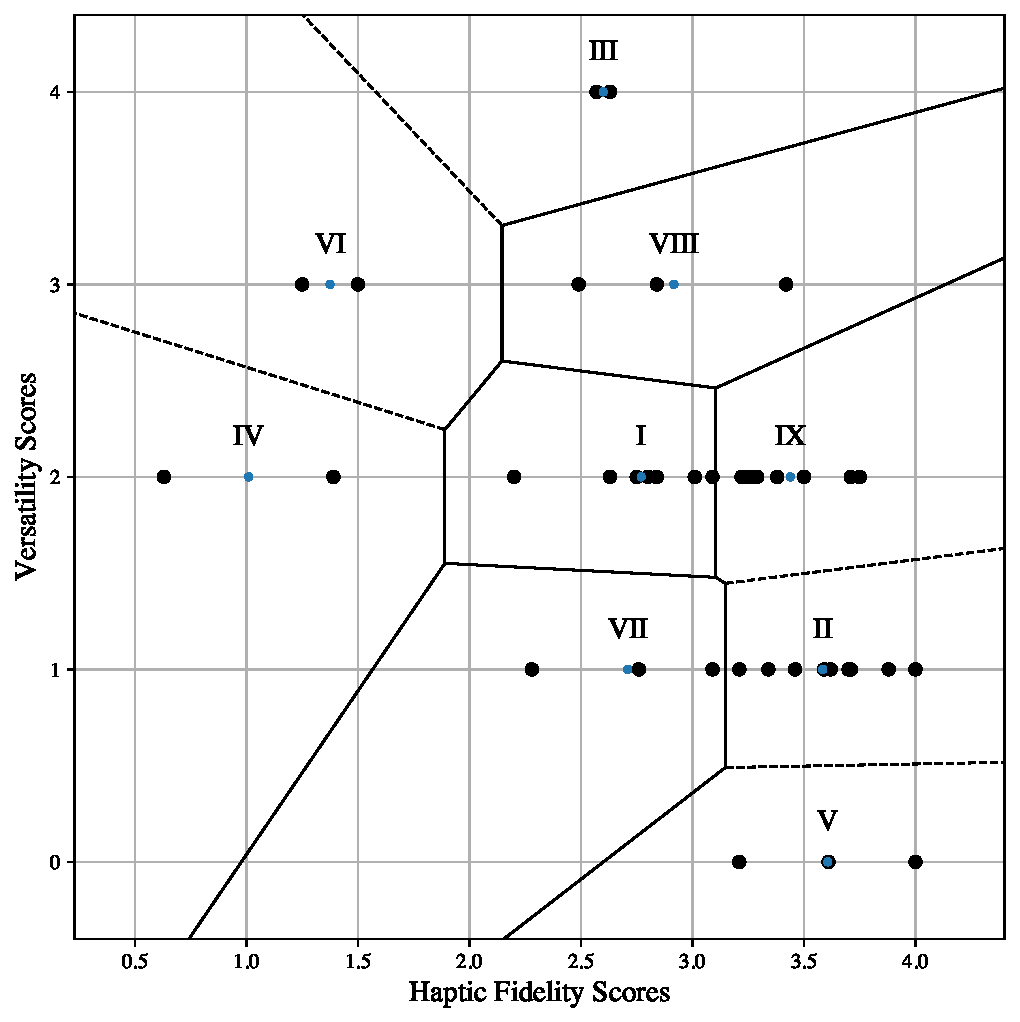
\includegraphics[width=\columnwidth]{literature_data.pdf} 
    \caption{KMeans clustering of the data}
    \label{fig:kmeans}
\end{figure}


\section{Discussion}
Suggestions: For the post hoc evaluation of the haptic feedback fidelity, it would be helpful if researchers included specifications of the device used, such as hard- and software latency, maximum force, sensor and actuator accuracy, etc., even if the device is commercially available. This makes the objective rating of the feedback fidelity easier and quicker, as even for commercially used devices the specifications might not be available anymore at some point in the future.

Often, an artificial task is chosen, such as tracking a trajectory with a steering wheel, where the velocity of the car is constant to eliminate the use of foot pedals \cite{LeeH2014}. For the retention, the subjects are using the exact same setup, so parameters such as the degrees of freedom, and the stimuli of experiment and retention are the same, thus increasing the level of fidelity. However, the performance of the participants driving a real car, or even driving in a more realistic simulator is never evaluated, despite this actually being the interesting question. In the end, we want to know how we can effectively improve motor learning performance by providing haptic feedback to the user. If we are doing this only for artificial tasks, we are making the experimental setup easier and possibly cheaper, but not exploring the greater possibilities this technology might offer. 

One important finding is that haptic feedback might be especially important when learning a motor task that requires 3 dimensions. Studies that required the participants to follow a trajectory in 2D have often found no significant improvement in task performance when providing haptic feedback, compared to visual feedback only (\cite{Gambaro2014}, \cite{LiuG2014}, \cite{LeeH2014}), whereas studies involving trajectory following in 3 dimensions have shown a significant improvement with the introduction of haptic feedback (\cite{Grant2019}, \cite{Rodriguez2010}, ...)


\onecolumn

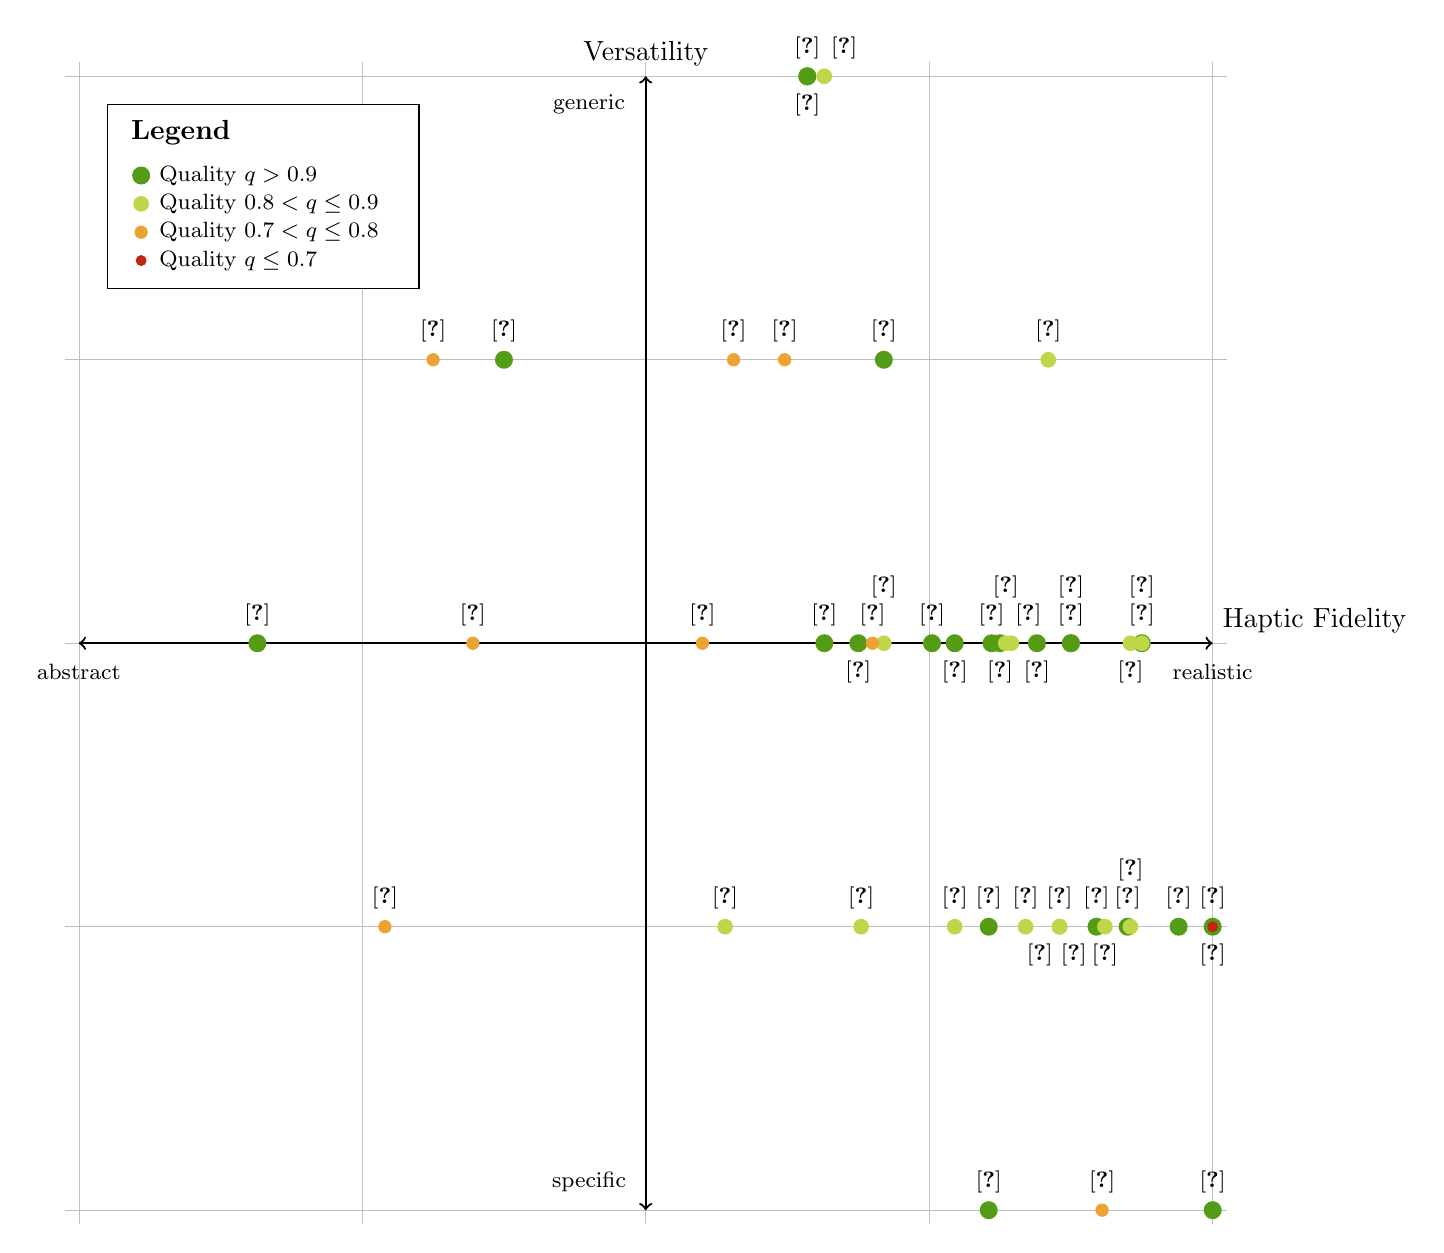
\begin{tikzpicture}[scale=3.6]
    
    % Add axis labels
    \foreach \x in {0,1,2,3,4} {
        \draw [very thin, lightgray](\x cm, 0-0.05) -- (\x cm, 4+0.05) node[anchor=north] {};
        \draw [very thin, lightgray](0-0.05,\x cm) -- (4+0.05,\x cm) node[anchor=east] {};
    }

    % Draw axes
    \draw[thick,<->] (0,2) -- (4,2) node[anchor=south west] {Haptic Fidelity};
    \draw[thick,<->] (2,0) -- (2,4) node[anchor=south] {Versatility};

    \node at (0,1.9) {\footnotesize{abstract}};
    \node at (4,1.9) {\footnotesize{realistic}};
    \node at (1.8,0.1) {\footnotesize{specific}};
    \node at (1.8,3.9) {\footnotesize{generic}};

    % Legend
    \draw[fill=white] (0.1,3.9) rectangle (1.2,3.25); % Legend border
    \node[anchor=west] at (0.15, 3.8) {\textbf{Legend}}; % Legend title
    
    \node[circle, fill=c1, inner sep=2.3pt] at (0.22, 3.65) {};
    \node[anchor=west] at (0.25, 3.65) {\footnotesize{Quality $q > 0.9$}};

    \node[circle, fill=c2, inner sep=2pt] at (0.22, 3.55) {};
    \node[anchor=west] at (0.25, 3.55) {\footnotesize{Quality $0.8 < q \leq 0.9$}};

    \node[circle, fill=c3, inner sep=1.7pt] at (0.22, 3.45) {};
    \node[anchor=west] at (0.25, 3.45) {\footnotesize{Quality $0.7 < q \leq 0.8$}};

    \node[circle, fill=c4, inner sep=1.4pt] at (0.22, 3.35) {};
    \node[anchor=west] at (0.25, 3.35) {\footnotesize{Quality $q \leq 0.7$}};
    
    % Sample data points
    \node[circle, fill=c1, inner sep=2.3pt] at (3.5,2) {};
    \node[circle, fill=c1, inner sep=2.3pt] at (3.22,2) {};
    \node[circle, fill=c1, inner sep=2.3pt] at (0.63,2) {};
    \node[circle, fill=c1, inner sep=2.3pt] at (3.38,2) {};
    \node[circle, fill=c1, inner sep=2.3pt] at (3.75,2) {};
    \node[circle, fill=c1, inner sep=2.3pt] at (2.63,2) {};
    \node[circle, fill=c1, inner sep=2.3pt] at (2.75,2) {};
    \node[circle, fill=c1, inner sep=2.3pt] at (3.21,0) {};
    \node[circle, fill=c1, inner sep=2.3pt] at (4,0) {};
    \node[circle, fill=c1, inner sep=2.3pt] at (4,1) {};
    \node[circle, fill=c1, inner sep=2.3pt] at (3.88,1) {};
    \node[circle, fill=c1, inner sep=2.3pt] at (1.5,3) {};
    \node[circle, fill=c1, inner sep=2.3pt] at (3.59,1) {};
    \node[circle, fill=c1, inner sep=2.3pt] at (3.09,2) {};
    \node[circle, fill=c1, inner sep=2.3pt] at (2.57,4) {};
    \node[circle, fill=c1, inner sep=2.3pt] at (3.21,1) {};
    \node[circle, fill=c1, inner sep=2.3pt] at (3.01,2) {};
    \node[circle, fill=c1, inner sep=2.3pt] at (3.25,2) {};
    \node[circle, fill=c1, inner sep=2.3pt] at (2.84,3) {};
    \node[circle, fill=c1, inner sep=2.3pt] at (3.7,1) {};
    \node[circle, fill=c1, inner sep=2.3pt] at (2.57,4) {};
    \node[circle, fill=c1, inner sep=2.3pt] at (3.5,2) {};
    \node[circle, fill=c2, inner sep=2.0pt] at (2.63,4) {};
    \node[circle, fill=c2, inner sep=2.0pt] at (2.84,2) {};
    \node[circle, fill=c2, inner sep=2.0pt] at (3.27,2) {};
    \node[circle, fill=c2, inner sep=2.0pt] at (3.34,1) {};
    \node[circle, fill=c2, inner sep=2.0pt] at (3.46,1) {};
    \node[circle, fill=c2, inner sep=2.0pt] at (3.46,1) {};
    \node[circle, fill=c2, inner sep=2.0pt] at (3.46,1) {};
    \node[circle, fill=c2, inner sep=2.0pt] at (3.62,1) {};
    \node[circle, fill=c2, inner sep=2.0pt] at (3.75,2) {};
    \node[circle, fill=c2, inner sep=2.0pt] at (3.09,1) {};
    \node[circle, fill=c2, inner sep=2.0pt] at (3.71,1) {};
    \node[circle, fill=c2, inner sep=2.0pt] at (3.29,2) {};
    \node[circle, fill=c2, inner sep=2.0pt] at (2.28,1) {};
    \node[circle, fill=c2, inner sep=2.0pt] at (3.42,3) {};
    \node[circle, fill=c2, inner sep=2.0pt] at (2.76,1) {};
    \node[circle, fill=c2, inner sep=2.0pt] at (3.71,2) {};
    \node[circle, fill=c3, inner sep=1.7pt] at (2.2,2) {};
    \node[circle, fill=c3, inner sep=1.7pt] at (2.8,2) {};
    \node[circle, fill=c3, inner sep=1.7pt] at (1.25,3) {};
    \node[circle, fill=c3, inner sep=1.7pt] at (1.39,2) {};
    \node[circle, fill=c3, inner sep=1.7pt] at (2.49,3) {};
    \node[circle, fill=c3, inner sep=1.7pt] at (3.61,0) {};
    \node[circle, fill=c3, inner sep=1.7pt] at (1.08,1) {};
    \node[circle, fill=c3, inner sep=1.7pt] at (2.31,3) {};
    \node[circle, fill=c4, inner sep=1.4pt] at (4,1) {};


    % Add citations to datapoints
    \node at (3.5,2.1) {\footnotesize{\cite{Brickler2019}}};
    \node at (3.22,2.1) {\footnotesize{\cite{Caccianiga2021}}};
    \node at (0.63,2.1) {\footnotesize{\cite{Crespo2015}}};
    \node at (3.38,1.9) {\footnotesize{\cite{Feygin2002HapticSkill}}};
    \node at (3.75,2.2) {\footnotesize{\cite{Feygin2002HapticSkill}}};
    \node at (2.63,2.1) {\footnotesize{\cite{Gambaro2014}}};
    \node at (2.75,1.9) {\footnotesize{\cite{Gambaro2014}}};
    \node at (3.21,0.1) {\footnotesize{\cite{Graham2008}}};
    \node at (4,0.1) {\footnotesize{\cite{Huang2006}}};
    \node at (4,1.1) {\footnotesize{\cite{Huang2007}}};
    \node at (3.88,1.1) {\footnotesize{\cite{LeeH2014}}};
    \node at (1.5,3.1) {\footnotesize{\cite{LiuH2019}}};
    \node at (3.59,1.1) {\footnotesize{\cite{Mohanty2023}}};
    \node at (3.09,1.9) {\footnotesize{\cite{Oquendo2024}}};
    \node at (2.57,3.9) {\footnotesize{\cite{Vasudevan2020}}};
    \node at (3.21,1.1) {\footnotesize{\cite{Dai2023}}};
    \node at (3.01,2.1) {\footnotesize{\cite{Dai2023}}};
    \node at (3.25,1.9) {\footnotesize{\cite{Gunter2022}}};
    \node at (2.84,3.1) {\footnotesize{\cite{LeeY2019}}};
    \node at (3.7,1.1) {\footnotesize{\cite{LiuG2014}}};
    \node at (2.57,4.1) {\footnotesize{\cite{McAnally2023}}};
    \node at (3.5,2.2) {\footnotesize{\cite{Rodriguez2010}}};
    \node at (2.7,4.1) {\footnotesize{\cite{Yang2023}}};
    \node at (2.84,2.2) {\footnotesize{\cite{Yang2023}}};
    \node at (3.27,2.2) {\footnotesize{\cite{Yang2023}}};
    \node at (3.34,1.1) {\footnotesize{\cite{Fehlberg2012}}};
    \node at (3.39,0.9) {\footnotesize{\cite{Fehlberg2012}}};
    \node at (3.51,0.9) {\footnotesize{\cite{Fehlberg2012}}};
    \node at (3.46,1.1) {\footnotesize{\cite{Fehlberg2012}}};
    \node at (3.62,0.9) {\footnotesize{\cite{Fehlberg2012}}};
    \node at (3.75,2.1) {\footnotesize{\cite{Fehlberg2012}}};
    \node at (3.09,1.1) {\footnotesize{\cite{Grant2019}}};
    \node at (3.71,1.2) {\footnotesize{\cite{Macuga2019}}};
    \node at (3.35,2.1) {\footnotesize{\cite{Morris2007}}};
    \node at (2.28,1.1) {\footnotesize{\cite{Najdovski2020}}};
    \node at (3.42,3.1) {\footnotesize{\cite{Oezen2022}}};
    \node at (2.76,1.1) {\footnotesize{\cite{Vaghela2021}}};
    \node at (3.71,1.9) {\footnotesize{\cite{Wall2000}}};
    \node at (2.2,2.1) {\footnotesize{\cite{Chappell2022}}};
    \node at (2.8,2.1) {\footnotesize{\cite{Chi2017}}};
    \node at (1.25,3.1) {\footnotesize{\cite{Hanashima2023}}};
    \node at (1.39,2.1) {\footnotesize{\cite{Perez2023}}};
    \node at (2.49,3.1) {\footnotesize{\cite{Trinitatova2023}}};
    \node at (3.61,0.1) {\footnotesize{\cite{Vaghela2021}}};
    \node at (1.08,1.1) {\footnotesize{\cite{Lee2012}}};
    \node at (2.31,3.1) {\footnotesize{\cite{Xia2023}}};
    \node at (4,0.9) {\footnotesize{\cite{Manivannan2008}}};

    
\end{tikzpicture}

\begin{table}[]
\begin{tabular}{@{}p{0.13\textwidth}p{0.08\textwidth}p{0.23\textwidth}p{0.19\textwidth}p{0.27\textwidth}@{}}
\toprule
 Feedback Fidelity & Reference & Experimental Design & Feedback Type & Findings \\ \midrule
 Low & \cite{Huang2007} &  &  & Auditory cues with feed-forward control do not help with task performance \\ \\
 Mid & \cite{Morris2007} & Follow trajectory with stylus & Haptic device with the opposite of the embedded force pattern & Performance was worse in haptic only compared to visual only, and far worse than visuo-haptic condition \\ \\
 High & \cite{Huang2007} & Maximum excitement of dynamic system with rotary handle at resonance frequency &  & decreased variance, increased precision \\ \bottomrule
\end{tabular}
\end{table}

\twocolumn

\section*{Appendix}

\subsection{Queries}
\label{sec:queries}

\subsubsection{Scopus}
TITLE-ABS-KEY (motor AND (learning OR control OR training OR skills) AND (((virtual OR augmented) AND reality) OR ((remote OR virtual OR simulated) AND environment)) AND (((somatosensory OR haptic OR tactile OR proprioceptive OR kinesthetic OR cutaneous OR somatic) AND (cue* OR feedback OR rendering OR stimul*)) AND (fidelity OR realism OR accuracy OR precision OR exactness OR specificity)))

\subsubsection{IEEE Xplore}
motor AND (learning OR control OR training OR skills) AND (((virtual OR augmented) AND reality) OR ((remote OR virtual OR simulated) AND environment)) AND (((somatosensory OR haptic OR tactile OR proprioceptive OR kinesthetic OR cutaneous OR somatic) AND (cue* OR feedback OR rendering OR stimuli*)) AND (fidelity OR realism OR accuracy OR precision OR exactness OR specificity)) 

\subsubsection{PubMed}
motor AND (learning OR control OR training OR skills) AND (((virtual OR augmented) AND reality) OR ((remote OR virtual OR simulated) AND environment)) AND (((somatosensory OR haptic OR tactile OR proprioceptive OR kinesthetic OR cutaneous OR somatic) AND (cue OR cues OR feedback OR rendering OR stimuli*)) AND (fidelity OR realism OR accuracy OR precision OR exactness OR specificity))


\bibliographystyle{IEEEtran}
\bibliography{references}


\end{document}
